\documentclass[tikz]{standalone}
\usepackage{tikz}
\usepackage{fourier}
\usepackage{physics}
\usetikzlibrary{shapes.geometric}
\usetikzlibrary{calc}
\usepackage{pgfplots}
\pgfplotsset{compat=1.18}

\begin{document}
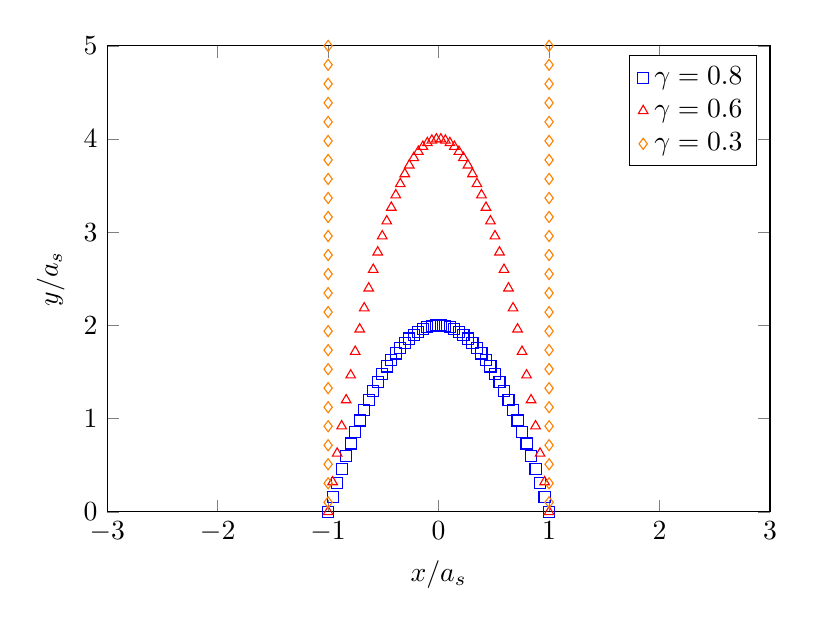
\begin{tikzpicture}
    \begin{axis}[
            width=10cm,height=7.5cm,
            xmin=-3,xmax=3,ymin=0,ymax=5,
            xlabel={\(x/a_s\)},
            ylabel={\(y/a_s\)},
        ]
        \addplot[only marks,blue,mark=square,samples=50, domain=-1.0:1.0]
        {-2*x^2 + 2};
        \addplot[only marks,red,mark=triangle,samples=50, domain=-1.0:1.0]
        {-4*x^2 + 4};
        \addplot[only marks, orange,mark=diamond,samples=50, domain=-1.0:1.0]
        ({-1}, {5 * x});
        \addplot[only marks, orange,mark=diamond,samples=50, domain=-1.0:1.0]
        ({1}, {5 * x});

        \addlegendentry{$\gamma = 0.8$}
        \addlegendentry{$\gamma = 0.6$}
        \addlegendentry{$\gamma = 0.3$}
    \end{axis}
\end{tikzpicture}
\end{document}